\documentclass[journal,12pt,twocolumn]{IEEEtran}

\usepackage{setspace}
\usepackage{gensymb}
\singlespacing
\usepackage[cmex10]{amsmath}

\usepackage{amsthm}

\usepackage{mathrsfs}
\usepackage{txfonts}
\usepackage{stfloats}
\usepackage{bm}
\usepackage{tcolorbox}
\usepackage{cite}
\usepackage{cases}
\usepackage{subfig}
\usepackage[T1]{fontenc}
\usepackage{inconsolata}

\usepackage{longtable}
\usepackage{multirow}

\usepackage{enumitem}
\usepackage{mathtools}
\usepackage{steinmetz}
\usepackage{tikz}
\usepackage{circuitikz}
\usepackage{verbatim}
\usepackage{tfrupee}
\usepackage[breaklinks=true]{hyperref}
\usepackage{graphicx}
\usepackage{tkz-euclide}
\usetikzlibrary{positioning}

\usetikzlibrary{calc,math}
\usepackage{listings}
    \usepackage{color}                                            %%
    \usepackage{array}                                            %%
    \usepackage{longtable}                                        %%
    \usepackage{calc}                                             %%
    \usepackage{multirow}                                         %%
    \usepackage{hhline}                                           %%
    \usepackage{ifthen}                                           %%
    \usepackage{lscape}     
\usepackage{multicol}
\usepackage{chngcntr}

\DeclareMathOperator*{\Res}{Res}

\renewcommand\thesection{\arabic{section}}
\renewcommand\thesubsection{\thesection.\arabic{subsection}}
\renewcommand\thesubsubsection{\thesubsection.\arabic{subsubsection}}

\renewcommand\thesectiondis{\arabic{section}}
\renewcommand\thesubsectiondis{\thesectiondis.\arabic{subsection}}
\renewcommand\thesubsubsectiondis{\thesubsectiondis.\arabic{subsubsection}}


\hyphenation{op-tical net-works semi-conduc-tor}
\def\inputGnumericTable{}                                 %%

\lstset{
%language=C,
frame=single, 
breaklines=true,
columns=fullflexible
}
\begin{document}


\newtheorem{theorem}{Theorem}[section]
\newtheorem{problem}{Problem}
\newtheorem{proposition}{Proposition}[section]
\newtheorem{lemma}{Lemma}[section]
\newtheorem{corollary}[theorem]{Corollary}
\newtheorem{example}{Example}[section]
\newtheorem{definition}[problem]{Definition}

\newcommand{\BEQA}{\begin{eqnarray}}
\newcommand{\EEQA}{\end{eqnarray}}
\newcommand{\define}{\stackrel{\triangle}{=}}
\bibliographystyle{IEEEtran}
\raggedbottom
\setlength{\parindent}{0pt}
\providecommand{\mbf}{\mathbf}
\providecommand{\pr}[1]{\ensuremath{\Pr\left(#1\right)}}
\providecommand{\qfunc}[1]{\ensuremath{Q\left(#1\right)}}
\providecommand{\sbrak}[1]{\ensuremath{{}\left[#1\right]}}
\providecommand{\lsbrak}[1]{\ensuremath{{}\left[#1\right.}}
\providecommand{\rsbrak}[1]{\ensuremath{{}\left.#1\right]}}
\providecommand{\brak}[1]{\ensuremath{\left(#1\right)}}
\providecommand{\lbrak}[1]{\ensuremath{\left(#1\right.}}
\providecommand{\rbrak}[1]{\ensuremath{\left.#1\right)}}
\providecommand{\cbrak}[1]{\ensuremath{\left\{#1\right\}}}
\providecommand{\lcbrak}[1]{\ensuremath{\left\{#1\right.}}
\providecommand{\rcbrak}[1]{\ensuremath{\left.#1\right\}}}
\theoremstyle{remark}
\newtheorem{rem}{Remark}
\newcommand{\sgn}{\mathop{\mathrm{sgn}}}
\providecommand{\abs}[1]{\left\vert#1\right\vert}
\providecommand{\res}[1]{\Res\displaylimits_{#1}} 
\providecommand{\norm}[1]{\left\lVert#1\right\rVert}
%\providecommand{\norm}[1]{\lVert#1\rVert}
\providecommand{\mtx}[1]{\mathbf{#1}}
\providecommand{\mean}[1]{E\left[ #1 \right]}
\providecommand{\fourier}{\overset{\mathcal{F}}{ \rightleftharpoons}}
%\providecommand{\hilbert}{\overset{\mathcal{H}}{ \rightleftharpoons}}
\providecommand{\system}{\overset{\mathcal{H}}{ \longleftrightarrow}}
	%\newcommand{\solution}[2]{\textbf{Solution:}{#1}}
\newcommand{\solution}{\noindent \textbf{Solution: }}
\newcommand{\cosec}{\,\text{cosec}\,}
\providecommand{\dec}[2]{\ensuremath{\overset{#1}{\underset{#2}{\gtrless}}}}
\newcommand{\myvec}[1]{\ensuremath{\begin{pmatrix}#1\end{pmatrix}}}
\newcommand{\mydet}[1]{\ensuremath{\begin{vmatrix}#1\end{vmatrix}}}
\numberwithin{equation}{subsection}
\makeatletter
\@addtoreset{figure}{problem}
\makeatother
\let\StandardTheFigure\thefigure
\let\vec\mathbf
\renewcommand{\thefigure}{\theproblem}
\def\putbox#1#2#3{\makebox[0in][l]{\makebox[#1][l]{}\raisebox{\baselineskip}[0in][0in]{\raisebox{#2}[0in][0in]{#3}}}}
     \def\rightbox#1{\makebox[0in][r]{#1}}
     \def\centbox#1{\makebox[0in]{#1}}
     \def\topbox#1{\raisebox{-\baselineskip}[0in][0in]{#1}}
     \def\midbox#1{\raisebox{-0.5\baselineskip}[0in][0in]{#1}}
\vspace{3cm}
\title{Assignment-1}
\author{Dasari Shree Ujjwal - EE18BTECH11010}
\maketitle
\newpage
\bigskip
\renewcommand{\thefigure}{\theenumi}
\renewcommand{\thetable}{\theenumi}
Github repository
\begin{lstlisting}
https://github.com/dsujjwal/C-DS
\end{lstlisting}
%
\section{\textbf{Problem}}
\textbf{Consider the following C Code Segment:}
\begin{tcolorbox}
\begin{verbatim}
a = b + c ;
e = a + 1 ;
d = b + c ;
f = d + 1 ;
g = e + f ;
\end{verbatim}
\end{tcolorbox}
In a compiler, this code segment is represented internally as a directed acyclic graph (DAG).The number of nodes in the DAG is $__$
\section{\textbf{Solution}}
\textbf{Answer:} 6.
\\~\\
DAG is a useful data structure for implementing transformations on \textbf{Basic Blocks}. A Basic Block is a straight line code sequence which has no branches in and out branches except to the entry and at the end respectively.It is a set of statements that always executes in a sequence one after the other. The code segment in the question is an example of a Basic Block.
A DAG is usually constructed using \textbf{Three-Address Codes}.
\\~\\

\textbf{General form of Three-Address Code:}

Three-address code is an intermediate code used by optimizing compilers to aid in the implementation of code-improving transformations.
The general form of a Three-Address Code is as follows:
\begin{center}\fbox{\textbf{a = b op c} }\end{center}

Here,
\\ 1) \textbf{a,b,c} are the operands which are constants,names or compiler generated temporaries.
\\ 2)  \textbf{op} represents operator

\textbf{Rules for construction of DAGs:} 

\textbf{Rule 1:} 
  In a DAG,Interior nodes always represent the operators.
    Exterior nodes (leaf nodes) always represent the names, identifiers or constants.

\textbf{Rule 2:}  While constructing a DAG, a check is made to find if there exists any node with the same value. A new node is created only when there does not exist any node with the same value.This action helps in detecting the common sub-expressions and avoiding the re-computation of the same.

\textbf{Rule 3:}  The assignment instructions of the form x:=y are not performed unless they are necessary.


\\~\\

\textbf{Construction of DAG:} 

1) The first step is drawing two nodes representing $b$ and $c$ ( Rule 1).
\begin{center}
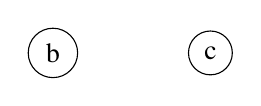
\begin{tikzpicture}

\path
(4.5,1) node [shape=circle,draw](a) {b}
(6.5,1) node [shape=circle,draw](b) {c};
\end{tikzpicture}

\end{center}

2) Now,we connect node $b$ and node $c$ to a new node $'+'$, completing the representation of Statement 1 of code (Rule 1 and 2).Since the node $'+'$ represents $a$ , we mention $a$ beside the node $'+'$ . 


\begin{center}
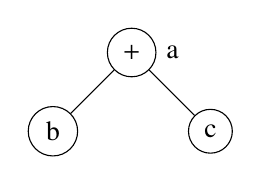
\begin{tikzpicture}
\path
(4.5,1) node [shape=circle,draw](a) {b}
(6.5,1) node [shape=circle,draw](b) {c}
(5.5,2) node [shape=circle,draw](c) {+};
\draw [-](a) --(c);
\draw [-](b) --(c);
\node [right] at (c.east) {a};

\end{tikzpicture}

\end{center}

3) Now,we make a new node $1$ and connect the new node $1$ and $'+'$ (representing $a$) to a new node $'+'$ (representing $e$), completing the representation of Statement 2 of code (Rule 1 and 2).Since the node $'+'$ represents $e$ , we mention $e$ besides the node.  
\begin{center}
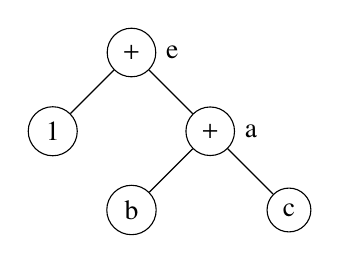
\begin{tikzpicture}
\path
(4.5,1) node [shape=circle,draw](a) {b}
(6.5,1) node [shape=circle,draw](b) {c}
(5.5,2) node [shape=circle,draw](c) {+}
(3.5,2) node [shape=circle,draw](d) {1}
(4.5,3) node [shape=circle,draw](e) {+};
\draw [-](a) --(c);
\draw [-](b) --(c);
\node [right] at (c.east) {a};
\draw [-](c) --(e);
\draw [-](d) --(e);
\node [right] at (e.east) {e};

\end{tikzpicture}

\end{center}

4) Statement 3 of the code is equivalent to Statement 1.So we don't make a new node for $d$ and just mention it beside $a$.Similarly Statement 4 of the code is equivalent to Statement 2.So we don't make a new node for $f$ and just mention it beside $e$.  

\begin{center}
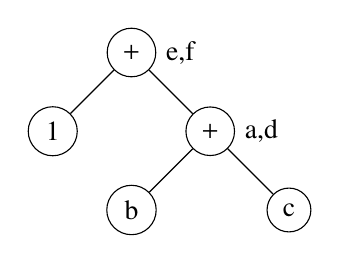
\begin{tikzpicture}
\path
(4.5,1) node [shape=circle,draw](a) {b}
(6.5,1) node [shape=circle,draw](b) {c}
(5.5,2) node [shape=circle,draw](c) {+}
(3.5,2) node [shape=circle,draw](d) {1}
(4.5,3) node [shape=circle,draw](e) {+};
\draw [-](a) --(c);
\draw [-](b) --(c);
\node [right] at (c.east) {a,d};
\draw [-](c) --(e);
\draw [-](d) --(e);
\node [right] at (e.east) {e,f};
\end{tikzpicture}

\end{center}

5) Now as $e$ and $f$ are same, we make a new node $g$ and connect it to $'+'$ (representing $e$ and $f$) using two edges. With this we have completed the representation of the complete code. 
\begin{center}
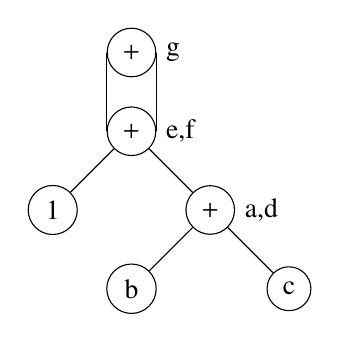
\begin{tikzpicture}
\path
(4.5,1) node [shape=circle,draw](a) {b}
(6.5,1) node [shape=circle,draw](b) {c}
(5.5,2) node [shape=circle,draw](c) {+}
(3.5,2) node [shape=circle,draw](d) {1}
(4.5,3) node [shape=circle,draw](e) {+}
(4.5,4) node [shape=circle,draw](f) {+};
\draw [-](a) --(c);
\draw [-](b) --(c);
\node [right] at (c.east) {a,d};
\draw [-](c) --(e);
\draw [-](d) --(e);
\node [right] at (e.east) {e,f};
\node [right] at (f.east) {g};
\draw [-] (e.west) --(f.west);
\draw [-] (e.east) --(f.east);

\end{tikzpicture}

\end{center}
Now can clearly see that the total number of nodes in the DAG is 6.
\end{document}
